\documentclass{standalone}
\usepackage{tikz}

\begin{document}
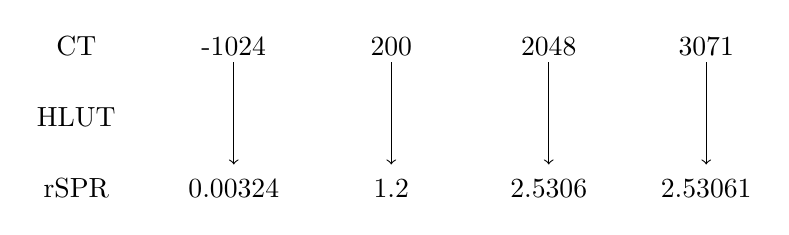
\begin{tikzpicture}

% Define row heights for shorter spacing
\def\rowa{1.8}
\def\rowb{0.9}
\def\rowc{0.0}

% First row - CT values
\node at (0, \rowa) {CT};
\node at (2, \rowa) {-1024};
\node at (4, \rowa) {200};
\node at (6, \rowa) {2048};
\node at (8, \rowa) {3071};

% Second row - HLUT with arrows pointing down
\node at (0, \rowb) {HLUT};
\draw[->] (2, \rowa - 0.2) -- (2, \rowc + 0.3);
\draw[->] (4, \rowa - 0.2) -- (4, \rowc + 0.3);
\draw[->] (6, \rowa - 0.2) -- (6, \rowc + 0.3);
\draw[->] (8, \rowa - 0.2) -- (8, \rowc + 0.3);

% Third row - rSPR values
\node at (0, \rowc) {rSPR};
\node at (2, \rowc) {0.00324};
\node at (4, \rowc) {1.2};
\node at (6, \rowc) {2.5306};
\node at (8, \rowc) {2.53061};

\end{tikzpicture}
\end{document}
